% !TEX root = USEGUIDE.tex

\part{CLASS : General overview}
\chapter{Generalities}
\section{Basic unit\label{sec:cSecond}}
All time in CLASS should be written in second. It corresponds to the cSecond, a CLASS c++ type, which are a \textbf{long long int} going, in 32 bits \textbf{and} 64 bits, up to  $(2^{63} - 1)~\textrm{s}~ \sim 2.9\cdot 10^{11}$ years, enough for any electro-nuclear scenarios one can consider....\\
 \section{CLASS working process principle}
image : sh�ma de principe de class
\chapter{Facilities descriptions}
All the facilities in CLASS project are regrouped inside a large group called CLASSFacility (and inherit of all the properties of the CLASSFacility in a C++ way). Inside the CLASSFacility, 3 different types has been defined, the reactor, the FabricationPlant (or more generally, all the fuel cycle front-end facilities) and the backend facilities. 
\section{CLASSFacility\label{sec:CLASSFacility}}
The CLASSFacility should never be used directly in the main CLASS program (the one made to perform the simulation).  The aim of these object is to regroup all the common properties of the nuclear facilities, such as common variables, methods, and builder. 


\section{Reactor\label{sec:reactor}}
\subsection{Generalities}
The aim of this class is to deal with the evolution of the fuel inside a reactor.\\
The evolution of the fuel is \textbf{always} contain in the \hyperref[sec:EvolutionData]{EvolutionData} \textit{fEvolutionDB}.\\
There are 2 way to provide the \hyperref[sec:EvolutionData]{EvolutionData} to the reactor. In the case of fixed fuel\footnote{Always the same input/output isotopic composition.} the user need to provide it, using the appropriated constructor, the set function, or a \hyperref[sec:CLASSFuelPlan]{CLASSFuelPlan}. In the case of recycled fuel or unfixed fuel, the user need to provide a \hyperref[sec:PhysicsModels]{PhysicsModels}, using the appropriated constructor, the set function, and/or a \hyperref[sec:CLASSFuelPlan]{CLASSFuelPlan}.

\subsection{Use}
There are 2 main ways to define a reactor, depending on the type of fuel loaded.

\subsubsection{Fixed Fuel}
Reactor using fixed fuel, which load always the same fresh fuel, and unload it with always the same burnup (same spent fuel...), to declare a reactor proceed as follow:
\begin{center}
\begin{minipage}{\textwidth}
\begin{lstlisting}
Reactor *MyReactor = new reactor(aCLASSLogger,		// CLASSLogger
				 myFuel_EvolutionData,	// EvolutionData
				 aBackEnd,		// BackEnd
				 myRe_StartingTime,	// Starting Time
				 myRe_LifeTime,		// Time of Life
				 myRe_Power,		// Power
				 myRe_HeavyMetalMass,	// HM mass
				 myRe_BurnUp,		// BurnUp
				 myRe_LoadFactor);	// LoadFactor
\end{lstlisting}
\end{minipage}
\end{center}
or
\begin{center}
\begin{minipage}{\textwidth}
\begin{lstlisting}
Reactor *MyReactor = new reactor(aCLASSLogger,		// CLASSLogger
				 myFuel_EvolutionData,	// EvolutionData
				 aBackEnd,		// BackEnd
				 myRe_StartingTime,	// Starting Time
				 myRe_LifeTime,		// Time of Life
				 myRe_CycleTime,	// Time of Cycle
				 myRe_HeavyMetalMass,	// HM mass
				 myRe_BurnUp);		// BurnUp
\end{lstlisting}
\end{minipage}
\end{center}
The meaning of each arguments of the two constructor previously defined are summed up in the following table

\begin{table}[H]
\begin{center}
\caption{Arguments of Reactor constructors}
\label{tab:meanKeyWord}
\begin{tabular}{|c|c|c|c|}
\hline
Argument & type & meaning & unit \\
\hline
aCLASSLogger 		&	\hyperref[sec:CLASSLogger]{CLASSLogger}		& Output messages 			& N.A.\\
myFuel\_EvolutionData	&	\hyperref[sec:EvolutionData]{EvolutionData}	& Fuel evolution description		& N.A. \\
aBackEnd 		&	\hyperref[sec:CLASSBackEnd]{CLASSBackEnd}	& Facility getting the spent fuel 	& N.A. \\
myRe\_StartingTime 	&	\hyperref[sec:cSecond]{cSecond}			& Creation time 			& second\\
myRe\_LifeTime 		&	\hyperref[sec:cSecond]{cSecond}			& Operation time 			& second\\
myRe\_Power 		&	double						& Thermal power 			& Watt\\
myRe\_HeavyMetalMass 	&	double						& Heavy metal mass 			& tons\\
myRe\_BurnUp 		&	double						& Burn up at EOC 			& GWd/tHM\\
myRe\_LoadFactor 	&	double						& Fraction of nominal power 		& .\\
myRe\_CycleTime 	&	\hyperref[sec:cSecond]{cSecond}			& the cycle time 			& second\\
\hline
\end{tabular}
\end{center}
\end{table}


\subsubsection{Reprocessed Fuel}
In this case, the fuel is provided by an external facility, so called, the \hyperref[sec:FabricationPlant]{FabricationPlant}. The way to build the reprocessed fresh fuel and to handle the fuel depletion calculation is done by the \hyperref[sec:PhysicsModels]{PhysicsModels}.
The main ways to defined a Reactor (with reprocessed fuel) is shown in the next two examples :

\begin{center}
\begin{minipage}{\textwidth}
\begin{lstlisting}
Reactor *MyReactor = new Reactor(aCLASSLogger,		// CLASSLogger
				 myFuel_PhysicsModels,	// PhysicsModels
				 aFabricationPlant,	// FabricationPlant
				 aBackEnd,		// BackEnd
				 myRe_StartingTime,	// Starting Time
				 myRe_LifeTime,		// Time of Life
				 myRe_Power,		// Power
				 myRe_HeavyMetalMass,	// HM mass
				 myRe_BurnUp,		// BurnUp
				 myRe_LoadFactor);	// LoadFactor
\end{lstlisting}
\end{minipage}
\end{center}
or
\begin{center}
\begin{minipage}{\textwidth}
\begin{lstlisting}
Reactor *MyReactor = new Reactor(aCLASSLogger,		// CLASSLogger
				 myFuel_PhysicsModels,	// PhysicsModels
				 aFabricationPlant,	// FabricationPlant
				 aBackEnd,		// BackEnd
				 myRe_StartingTime,	// Starting Time
				 myRe_LifeTime,		// Time of Life
				 myRe_CycleTime,	// Time of Cycle
				 myRe_HeavyMetalMass,	// HM mass
				 myRe_BurnUp);		// BurnUp
\end{lstlisting}
\end{minipage}
\end{center}
The meaning of each arguments of the two constructor previously defined are summed up in the following table

\begin{table}[H]
\begin{center}
\caption{Arguments of Reactor constructors}
\label{tab:meanKeyWord}
\begin{tabular}{|c|c|c|c|}
\hline
Argument & type & meaning & unit \\
\hline
aCLASSLogger 		& \hyperref[sec:CLASSLogger]{CLASSLogger}		& Output messages 			& N.A.\\
myFuel\_PhysicsModels	& \hyperref[sec:PhysicsModels]{PhysicsModels}		& Fuel construction/evolution		& N.A. \\
aFabricationPlant 	& \hyperref[sec:FabricationPlant]{FabricationPlant}	& Facility building the fuel 		& N.A. \\
aBackEnd 		& \hyperref[sec:CLASSBackEnd]{CLASSBackEnd}		& Facility getting the spent fuel 	& N.A. \\
myRe\_StartingTime 	& \hyperref[sec:cSecond]{cSecond}			& Creation time 			& second\\
myRe\_LifeTime 		& \hyperref[sec:cSecond]{cSecond}			& Operation time 			& second\\
myRe\_Power 		& double						& Thermal power 			& Watt\\
myRe\_HeavyMetalMass 	& double						& Heavy metal mass 			& tons\\
myRe\_BurnUp 		& double						& Burn up at EOC 			& GWd/tHM\\
myRe\_LoadFactor 	& double						& Fraction of nominal power 		& .\\
myRe\_CycleTime 	& \hyperref[sec:cSecond]{cSecond}			& the cycle time 			& second\\
\hline
\end{tabular}
\end{center}
\end{table}


\section{CLASSBackEnd\label{sec:CLASSBackEnd}}
The CLASSBackEnd class is a master class which aims to regroup all common properties of the fuel back-end facilities. All other back-end facilities in CLASS inherit of the CLASSBackEnd.\\
In CLASS, a CLASSBackEnd does not control its upstream. Its incoming material flux is pushed by its upstream facility (a Reactor, or an other CLASSBackEnd). It only controls its downstream flux.\\
\textbf{This object is not supposed to be used explicitly in a CLASS input.}
\subsection{Storage}
Storage is a CLASSBack end without associated downstream factory. All the incoming material are stored individually. During the storage, the depletion by decay is taken into account. The storage has to be defined as follow :
\begin{center}
\begin{minipage}{\textwidth}
\begin{lstlisting}
Storage *Stock = new Storage(aCLASSLogger);
\end{lstlisting}
\end{minipage}
\end{center}
 
 
\subsection{Pool\label{sec:pool}}
Pool is a CLASSBack end with an associated downstream factory. All incoming material will be pushed in the downstream factory after a set time, so called CoolingTime. All the incoming material are stored individually. During the cooling process, the depletion by decay is taken into account. The storage has to be defined as follow :
\begin{center}
\begin{minipage}{\textwidth}
\begin{lstlisting}
Pool *MyPool = new Pool(aCLASSLogger, aCLASSBackEnd, 5*365.25*24.*3600);
\end{lstlisting}
\end{minipage}
\end{center}
In the previous example, a 5 years cooling time has been used.
If no downstream facility is set, all the material will be pushed after cooling to the WASTE of the Scenario. To do so :
\begin{center}
\begin{minipage}{\textwidth}
\begin{lstlisting}
Pool *MyPool = new Pool(aCLASSLogger, 5*365.25*24.*3600);
\end{lstlisting}
\end{minipage}
\end{center}

\subsection{SeparationPlant\label{sec:SeparationPlant}}
The role of the SeparationPlant is to separate an incoming \hyperref[sec:IsotopicVector]{IsotopicVector} from a facility into an arbitrary number of outgoing \hyperref[sec:CLASSBackEnd]{CLASSBackEnd}.\\
To define a SeparationPlant proceed as follow :
\begin{center}
\begin{minipage}{\textwidth}
\begin{lstlisting}
SeparationPlant* MySeparationPlant = new SeparationPlant(aCLASSLogger);
\end{lstlisting}
\end{minipage}
\end{center}

The separation process is instantaneous and it follow the isotopic separation efficiency. It must be given as an IsotopicVector containing the separation efficiency for each nucleus. Note that it is possible to separate the incoming \hyperref[sec:IsotopicVector]{IsotopicVector} in many, the users must provide as many isotopic separation efficiency as outgoing \hyperref[sec:CLASSBackEnd]{CLASSBackEnd}.\\
In addition of a outgoing CLASSBackEnd and an associated isotopic separation efficiency, the user must provide a date for the separation to be effective. To do so :
\begin{center}
\begin{minipage}{\textwidth}
\begin{lstlisting}
IsotopicVector IV_MA;
IV_MA.Add(93, 237, 0, 1.);
IV_MA.Add(95, 242, 1, 1.);
IV_MA.Add(96, 245, 0, 1.);
//...
MySeparationPlant->SetBackEndDestination(aCLASSBackEnd1, 
					IV_MA, 
					2000*365.25*24.3600);

IsotopicVector IV_Pu;
IV_Pu.Add(94, 238, 0, 0.8);
IV_Pu.Add(94, 239, 0, 0.8);
//...
MySeparationPlant->SetBackEndDestination(aCLASSBackEnd2, 
					IV_Pu, 
					2005*365.25*24.3600);
					
IsotopicVector IV_U;
IV_U += 0.5*ZAI(92, 235, 0);
IV_U += 0.5*ZAI(92, 238, 0);
//...
MySeparationPlant->SetBackEndDestination(aCLASSBackEnd3, 
					IV_U, 
					2015*365.25*24.3600);
\end{lstlisting}
\end{minipage}
\end{center}
In the present example, the separation of Minor Actinides start in 2000 sending it to the CLASSBackEnd \textit{aCLASSBackEnd1} (the rest going to the WASTE). The separation of the plutonium start in 2005 (send in the \textit{aCLASSBackEnd2}) and the separation of uranium in 2010.\\
Note that between 2005 and 2010, both MA and Pu are separated and sent respectively to \textit{aCLASSBackEnd1} and \textit{aCLASSBackEnd2}, all the remaining isotopes are sent to the WASTE. After 2010, MA, Pu and U are separated and sent to their respective CLASSBackEnd facilities, the rest is still send to WASTE.\\
Furthermore, the separation of Actinides Minor has an efficiency of 100\%, Pu of 80\% and U of 50\%.

\section{Fabrication Plant\label{sec:FabricationPlant}}
The FabricationPlant is the facility which takes care about the fuel Fabrication. The "action" in FabricationPlant appends before the beginning of Cycle of a reactor: One fabrication time (Fabrication duration) before the BOC, it start the building process of the fuel.\\
First it sort the different stock in the different input Storage according the users priority. Then take the EquivalenceModel in PhysicsModels of the reactor, ask it how to build a fuel with the correct properties using some stock available. The EquivalenceModel provide a list a fraction to take in each stock. According to this fraction list, the FabricationPlant take the fraction is each stock and build the reprocessed fuel.
Once the reprocess fuel is made, it ask to the PhyscisModel to calculate its evolution and store it in EvolutionData form until the reactor load the fuel.\\
Between the fuel fabrication and the fuel loading in the reactor, the deplay through decay of the fuel is of course taking into account.\\
Note that, the FabricationPlant provide to the EquivalenceModel a list of stock which have virtually decay during the fabrication time in order to build a proper fuel.

To setup a FabricationPlant do as follow :
\begin{center}
\begin{minipage}{\textwidth}
\begin{lstlisting}
FabricationPlant *MyFabricationPlant = new FabricationPlant(gCLASS->GetLog(), 1*year);
MyFabricationPlant->SetFiFo();
\end{lstlisting}
\end{minipage}
\end{center}

In the previous example, the SetFifo() method set the first in first out priority for the stock usage.

One must also provide a list of Storage used to extract the Fissile part of the fuel by using :
\begin{center}
\begin{minipage}{\textwidth}
\begin{lstlisting}
MyFabricationPlant->AddFissileStorage(Stock);
\end{lstlisting}
\end{minipage}
\end{center}
And if necessary it is possible to storage to extract fertile isotopes using :
\begin{center}
\begin{minipage}{\textwidth}
\begin{lstlisting}
MyFabricationPlant->AddFertileStorage(Stock);
\end{lstlisting}
\end{minipage}
\end{center}
If no Fertile Storage are defined, the fertile part is taken from outside of the Scenario.
By default the unuse part of the stock is send to WASTE.But it is possible to set a storage where the unuse part of the stock using :
\begin{center}
\begin{minipage}{\textwidth}
\begin{lstlisting}
MyFabricationPlant->SetReUsableStorage(ReUsable);
\end{lstlisting}
\end{minipage}
\end{center}

\section{PathWay between Faiclity}
As explain previously, there are 3 different facility family, the FabricationPlant, the reactor, and the CLASSBackEnd.
The CLASSBackEnd facilities can't pull material inside, there is always a other facility which push material inside the CLASSBackEnd, but some can also push material inside other facilities: the SeparationPlant and the Pool. The Storage can only store materials.\\
The reactor take is fuel in a FabricationPlant and push the irradiated fuel in a CLASSBackEnd.\\
The FabricationPlant take its materials inside storage and stock the reprocessed fuel its makes unties the BoC.
We propose in the following 4 example of pathway between difference facilities. The point here is only to illustrated possible pathway, but the illustration may not be exhaustive. Furthermore, almost any composition between these examples could be made.


\subsection{Reactor with fixed fuel and a Storage}
\begin{figure}[h!]
\centering
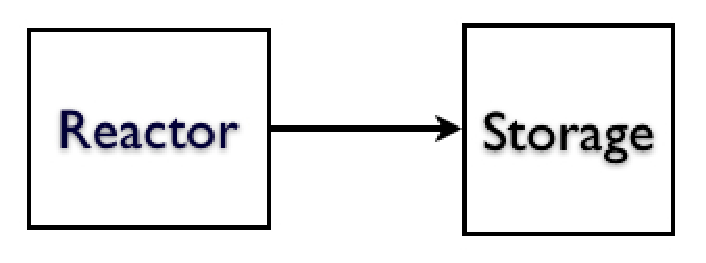
\includegraphics[width=0.4\textwidth]{R-S} 
\caption{Shematic Pathway\label{fig:R-S} }
\end{figure}
\begin{center}
\begin{minipage}{\textwidth}
\begin{lstlisting}
CLASSLogger *Logger = new CLASSLogger("CLASS_OUTPUT.log",1,2);  
EvolutionData* myFuel_EvolutionData = new EvolutionData(Logger, "/PATH/EvolData.dat");

Storage* MyStorage = new Storage(Logger);

Reactor *MyReactor = new Reactor(Logger, myFuel_EvolutionData, MyStorage, 0, 40*365.25*24.3600, 900E6, 100, 45, 1);	
\end{lstlisting}
\end{minipage}
\end{center}

\subsection{Reactor with fixed fuel, a Pool and a Storage}
\begin{figure}[h!]
\centering
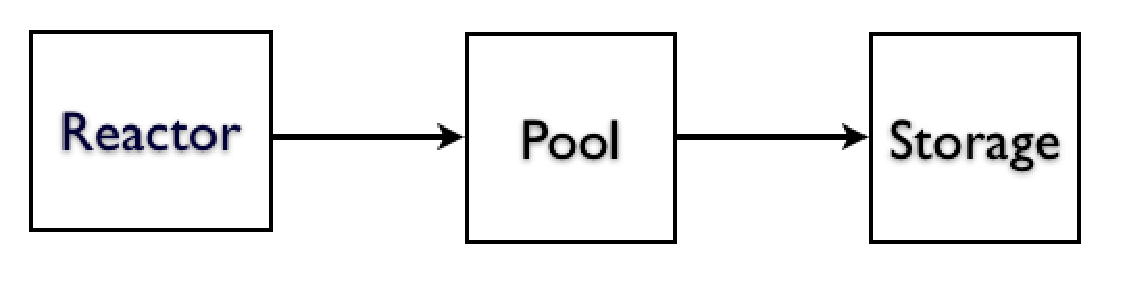
\includegraphics[width=0.6\textwidth]{R-P-S} 
\caption{Shematic Pathway\label{fig:R-P-S} }
\end{figure}

\begin{center}
\begin{minipage}{\textwidth}
\begin{lstlisting}
CLASSLogger *Logger = new CLASSLogger("CLASS_OUTPUT.log",1,2);  
EvolutionData* myFuel_EvolutionData = new EvolutionData(Logger, "/PATH/EvolData.dat");

Storage* MyStorage = new Storage(Logger);
Pool* MyPool = new Pool(Logger, MyStorage, 5*365.25*24*3600);

Reactor *MyReactor = new Reactor(Logger, myFuel_EvolutionData, MyPool, 0, 40*365.25*24.3600, 900E6, 100, 45, 1);	
\end{lstlisting}
\end{minipage}
\end{center}

\subsection{Reactor with fixed fuel, two SeprationPlant, a Pool and four Storage}
\begin{figure}[h!]
\centering
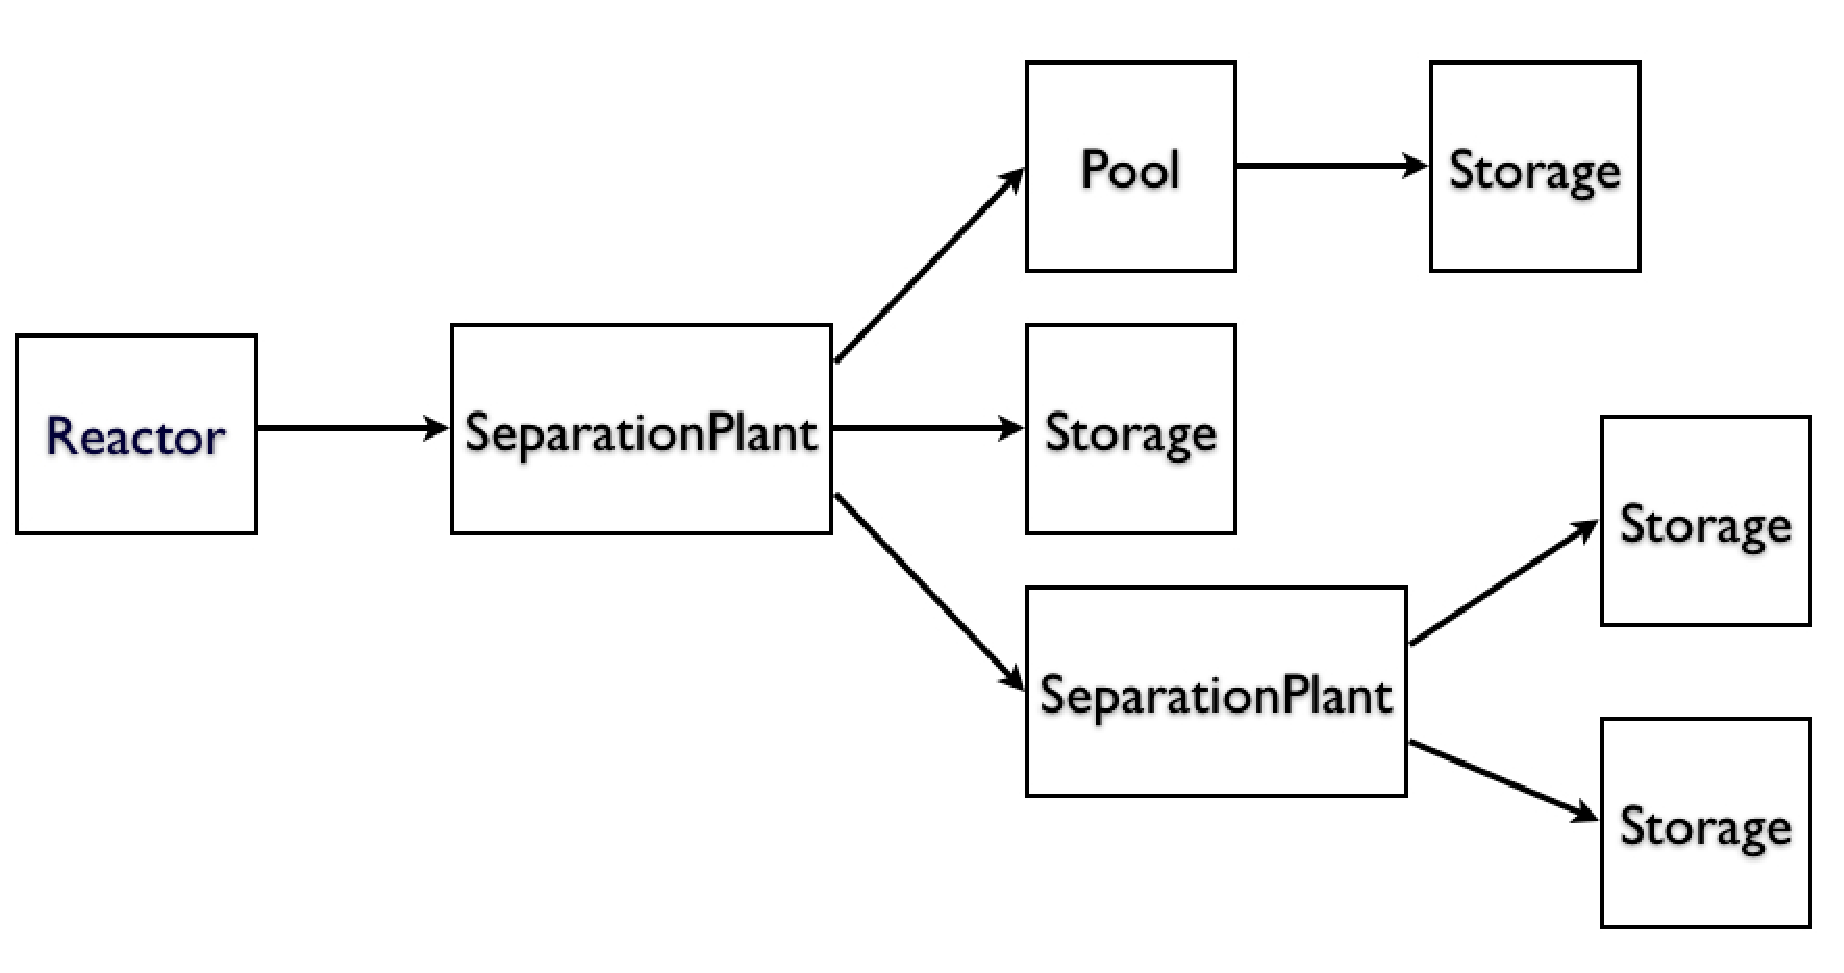
\includegraphics[width=1\textwidth]{R-SP-P_S-S-SP_S_S} 
\caption{Shematic Pathway\label{fig:R-SP-P_S-S-SP_S_S} }
\end{figure}
\begin{center}
\begin{minipage}{\textwidth}
\begin{lstlisting}
CLASSLogger *Logger = new CLASSLogger("CLASS_OUTPUT.log",1,2);  
EvolutionData* myFuel_EvolutionData = new EvolutionData(Logger, "/PATH/EvolData.dat");

Storage* MyStorage1 = new Storage(Logger);
Storage* MyStorage2 = new Storage(Logger);
Storage* MyStorage3 = new Storage(Logger);
Storage* MyStorage4 = new Storage(Logger);

Pool* MyPool1 = new Pool(Logger, MyStorage1, 5*365.25*24*3600);

// SeparationPlant separate U5 from U8 which goes in Storage 3 and 4.
SeparationPlan* MySeparation1 = new SeparationPlant(Logger);
IsotopicVector IV_U8;
IV_U8.Add(92, 238, 0, 1);
MySeparationPlant1->SetBackEndDestination(MyStorage3, IV_U8, 0);
					
IsotopicVector IV_U5;
IV_U5 += 1*ZAI(92, 235, 0);
MySeparationPlant1->SetBackEndDestination(MyStorage4, IV_U5, 0);
					

// SeparationPlant separate Am Pu and U which goes respectively in myPool1, myStorage2 and mySeparationPlan1.
SeparationPlan* MySeparation2 = new SeparationPlant(Logger);
IsotopicVector IV_MA;
IV_MA.Add(95, 242, 1, 1.);
MySeparationPlant2->SetBackEndDestination(MyPool1, IV_MA, 0);

IsotopicVector IV_Pu;
IV_Pu.Add(94, 239, 0, 0.8);
MySeparationPlant2->SetBackEndDestination(MyStorage2, IV_Pu, 0);
					
IsotopicVector IV_U;
IV_U.Add(92, 238, 0, 0.5);
IV_U.Add(92, 235, 0, 0.5);
MySeparationPlant2->SetBackEndDestination(MySeparationPlant1, IV_U, 0);

Reactor *MyReactor = new Reactor(Logger, myFuel_EvolutionData, MySeparation2, 0, 40*365.25*24.3600, 900E6, 100, 45, 1);	

\end{lstlisting}
\end{minipage}
\end{center}


\subsection{Reactor, a FabricationPlant, a Pool and a Storage}


\begin{center}
\begin{minipage}{\textwidth}
\begin{lstlisting}
CLASSLogger *Logger = new CLASSLogger("CLASS_OU TPUT.log",1,2);  

IM_RK4 *IMRK4 = new IM_RK4(Logger);
EQM_LIN_PWR_MOX* EQMLINPWRMOX = new EQM_LIN_PWR_MOX(Logger, "/PATH/EQ_Lin.dat");
EQM_QUAD_PWR_MOX* EQMQUADPWRMOX = new EQM_QUAD_PWR_MOX(Logger, "/PATH/DBParam.dat");
PhysicsModels* myFuel_PhysicsModel = new PhysicsModels(XSMOX, EQMQUADPWRMOX, IMRK4);

Storage* MyStorage = new Storage(Logger);
Pool* MyPool = new Pool(Logger, MyStorage, 5*365.25*24*3600);

FabricationPlant* myFabrication = new FabricationPlant(Logger, 2*365.25*24*3600);

Reactor *MyReactor = new Reactor(Logger, myFuel_PhysicsModel, myFabrication, MyPool, 0, 40*365.25*24.3600, 900E6, 100, 45, 1);	
\end{lstlisting}
\end{minipage}
\end{center}
\begin{figure}[h!]
\centering
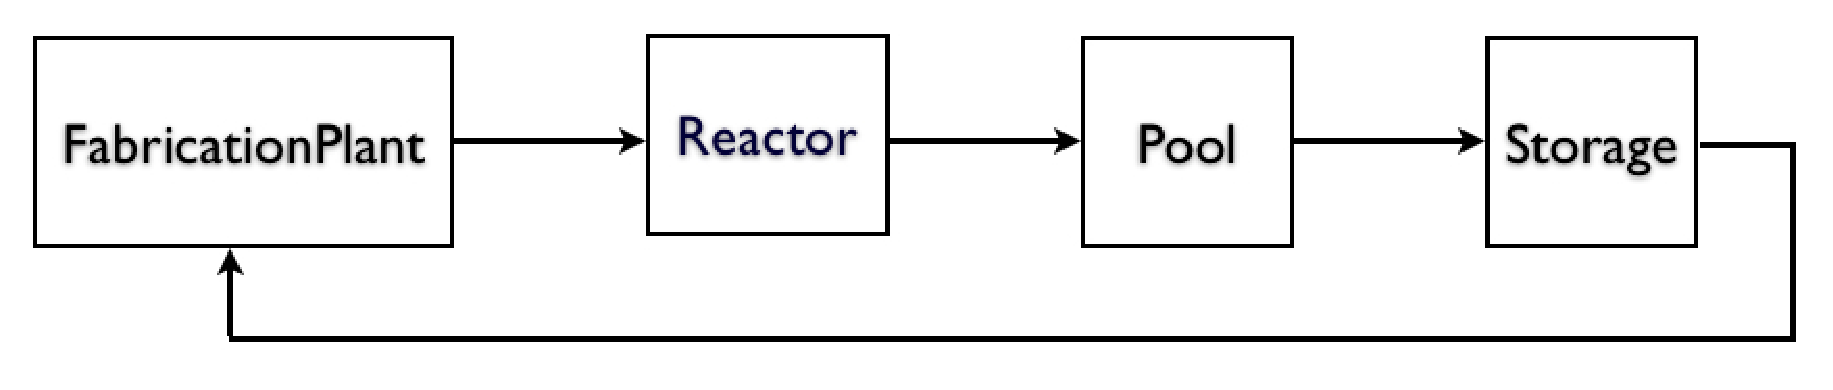
\includegraphics[width=0.9\textwidth]{FP_R_P_S} 
\caption{Shematic Pathway\label{fig:FP_R_P_S} }
\end{figure}

\chapter{Other objects}
\section{ZAI\label{sec:ZAI}}
The ZAi object represents a nucleus, from its charge number, mass number and isomeric state.\\
The object save  the charge number Z, the mass number A and the isomeric state I  of a nucleus : I=0 for ground state , I=1 for the first isomeric state ...\\
To declare a ZAI object proceed as follow :
\begin{center}
\begin{minipage}{\textwidth}
\begin{lstlisting}
ZAI U238 = ZAI(92, 238, 0);
\end{lstlisting}
\end{minipage}
\end{center}
This class includes the mains logical comparators (\emph{e.g} ==, >, !=). Fill free to read the doxygen for more details on the methods associated to this class. (\emph{e.g} A(), Z(), I(), N()...) \cite{doxygen}.
%\vspace{4cm}

\section{IsotopicVector\label{sec:IsotopicVector}}
\subsection{Generality}
The IsotopicVector object is a collection of ZAI, for each ZAI a number of nuclei is associated (IsotopicVector is a c++ map of ZAI and double, which corresponds to a sorted array of ZAI and its quantity).\\
Two pincipales operation have been defined on IsotopicVector. 
The following illustrates the possible operation allowed for IsotopicVectors :
\paragraph{Definiton \& Addition of nuclei}
\begin{center}
\begin{minipage}{\textwidth}
\begin{lstlisting}
IsotopicVector IV_1;
IsotopicVector IV_2;

IV_1 += 23 * ZAI(92, 238, 0); // Add 23 nucleus of uranium 238 to ZAI_1
IV_1 += 52 * ZAI(92, 235, 0); // Add 52 nucleus of uranium 235 to ZAI_1
\end{lstlisting}
\end{minipage}
\end{center}
\paragraph{Multiplication}
\begin{center}
\begin{minipage}{\textwidth}
\begin{lstlisting}
IV_1 *= 100; // Multiply all the nuclei quantities by 100 -> resulting : 2300 uranium 238 and 5200 uranium 235

IV_2 = IV_1 * 10; // IV_2 will be equal to 10 IV_1 
\end{lstlisting}
\end{minipage}
\end{center}
\paragraph{Sum}
\begin{center}
\begin{minipage}{\textwidth}
\begin{lstlisting}
IsotopicVector IV_sum = IV_1 + IV2; // IV_sum will be equal to 11 IV_1
\end{lstlisting}
\end{minipage}
\end{center}

Some additional operations have been also implemented, such as subtraction. It works as the sum, but if the result of the subtraction is negative for some nuclei, those nuclei are set to zero and the difference is added to the, so called, \textit{fIsotopicQuantityNeeded}. If so, a WARNING will be written on the terminal.\\
@@ Link WARNING \\
\textbf{To insure the quality and the reliability of the simulation, the fIsotopicQuantityNeeded MUST remain empty.}


\subsection{Print method}
You can use the Print() method to write the composition of an IsotopicVector.
When printing the IsotopicVector composition present nuclei, as well as the \textit{needed} one, are written with their corresponding quantity (unit: nucleus number).\\


\subsection{GetTotalMass}
Return the mass of the IsotopicVector in tons using :
\begin{center}
\begin{minipage}{\textwidth}
\begin{lstlisting}
double TotalMass = IV.GetTotalMass();
\end{lstlisting}
\end{minipage}
\end{center}


\subsection{Multiplication between IsotopicVector}
The result of this operation is an IsotopicVector, where each nucleus quantity is the product of the corresponding nucleus quantity of the two IsotopicVector.\\
In other words :\\
If a nucleus A is present in both IsotopicVector, with respective quantity $\alpha$ and $\beta$, the resulting IsotopicVector will contain $\alpha\times\beta$ nucleus A. If the nucleus A is not present in both IsotopicVector, the resulting IsotopicVector will not contain the nucleus A.\\

\textit{By exemple, this method can be used to apply separation efficiency: one IsotopicVector containing real material and the other one containing separation efficiency of each nucleus.}

\section{EvolutionData}\label{sec:EvolutionData}
An EvolutionData aims to describe the evolution of an \hyperref[sec:IsotopicVector]{IsotopicVector} through a physical process (decay or irradiation). The Decay case is fully described in section~\ref{sec:DecayDB}.\\

In case of irradiation, it may also contains the evolution of the one group cross section, the evolution of the neutron flux and the keff and are not mandatory. Note that neutron flux and keff are not used in CLASS. The EvolutionData MUST contain the power and can contain the heavy metal mass, the fuel type, reactor type and the cycle time.\\
These EvolutionData can be loaded into CLASS from a formatted ASCII file see section~\ref{sec:EDformat} as follow :

\begin{center}
\begin{minipage}{\textwidth}
\begin{lstlisting}
CLASSLogger *Logger = new CLASSLogger("CLASS_OUTPUT.log",1,2);  
 
EvolutionData*  MyEvolutionData = new EvolutionData(Logger, "/PATH/Data.dat");
\end{lstlisting}
\end{minipage}
\end{center}


\subsection{EvolutionData ASCII format}\label{sec:EDformat}
The formatted ASCII file describing the EvolutionData is formatted as follow:
\begin{center}
\begin{minipage}{\textwidth}
\begin{lstlisting}[label=lst:DatFormat,caption=Evolution Data format]
time "0 t2 t3 ..."						// in seconds
keff "k1 k2 k3 ..."					// not mandatory entry
flux "phi1 phi2 phi3 ..." 			//(neutron/(second.cm2))not mandatory entry
Inv "Z A I inv1 inv2 inv 3 ..."		//in atoms
...
XSFis "Z A I xsfis1 xsfis2 xsfis3 ..."//in barns
... 
XSCap "Z A I xscap1 xscap2 xscap3 ..."
...
XSn2n "Z A I xsn2n1 xsnsn2 xsn2n3 ..."
...
\end{lstlisting}
\end{minipage}
\end{center}

The meaning of each keyword is listed in table~\ref{tab:meanKeyWord}.

\begin{table}[H]
\begin{center}
\caption{.dat Key words meaning}
\label{tab:meanKeyWord}
\begin{tabular}{|c|c|}
\hline
Key words & Meaning \\
\hline
Inv & Inventory \\
\hline
XSFis &   fission cross section \\
XSCap & $(n,\gamma)$ cross section\\
XSn2n  &  $(n,2n)$ cross section \\
\hline
\hline
Value & meaning \\
\hline
Z & Charge number\\
A & Mass number\\
I & State (fundamental=0, $1^{st}$ excited =1, ...) \\
\hline
\end{tabular}
\end{center}

\end{table}

Each EvolutionName.dat files comes with a EvolutionName.info file, which describes the reactor, it is formatted like this :

\begin{center}
\begin{minipage}{\textwidth}
\begin{lstlisting}
Reactor "ReactorName"		//What ever string without space
Fueltype "FuelName"			//What ever string without space
CycleTime "t"						//The final time simulated (@@BaM)
ConstantPower "P"				//Simulated power (in W)
\end{lstlisting}
\end{minipage}
\end{center}


\subsection{DecayDataBank}\label{sec:DecayDB}
The radioactive decay is handled by a DecayDataBank. The DecayDataBank contains an EvolutionData for each nucleus of the nuclei chart. 
Each EvolutionData describes the evolution of the nucleus and all its daughters as a function of the time. The depletion of an isotopic vector corresponds to the sum of all its nucleus depletion contribution.\\

In other words, in CLASS, for each nucleus of the chart, a depletion calculation has been performed and compiled in a DecayDataBank.\\
The determination  of an \hyperref[sec:IsotopicVector]{IsotopicVector} depletion is performed as follow :\\
First, one determines the depletion of each nucleus of the \hyperref[sec:IsotopicVector]{IsotopicVector} following the DecayDataBank, then sums all those contributions.

DecayDataBank can be defined as follow :

\begin{center}
\begin{minipage}{\textwidth}
\begin{lstlisting}
CLASSLogger *Logger = new CLASSLogger("CLASS_OUTPUT.log",1,2);

DecayDataBank* DecayDB = new DecayDataBank(Logger, "/PATH/Decay.idx");
\end{lstlisting}
\end{minipage}
\end{center}
In the previous example a DecayDataBank has been defined using the file Decay.idx file. This file lists all the path to EvolutionDatas (each one corresponding to the depletion of one nucleus). The format of the .idx file is the following :

\begin{center}
\begin{minipage}{\textwidth}
\begin{lstlisting}
Z1 A1 I1 PATH/ZAI1.dat
...
Zn An In PATH/ZAIn.dat
\end{lstlisting}
\end{minipage}
\end{center}
A DecayDataBank can be find in \$PATH\_TO\_CLASS/Data/@@@.


\section{Log management : CLASSLogger}\label{sec:CLASSLogger}
In CLASS, all messages are handled by the CLASSLogger object. There are 4 verbose levels, see table~\ref{tab:verblevel}.

\begin{table}[H]
\begin{center}
\caption{Verbose levels}
\label{tab:verblevel}
\begin{tabular}{|c|c|l|}
\hline
level \# & meaning & informations\\
\hline
0 & ERROR & This is the default. \textit{It makes the code to stop}\\
\hline
1 & WARNING & LVL 0 + something may go wrong but the code continue running\\
\hline
2 & INFO &  LVL 1 + simple informations about ongoing process \\
\hline
3 & DEBUG & LVL 2 + each method begin and end \\
\hline
\end{tabular}
\end{center}
\end{table}

There are two outputs for these messages : the standard output (terminal) and a logfile. For each output a verbose level can be assigned as follow :
\begin{center}
\begin{minipage}{\textwidth}
\begin{lstlisting}
CLASSLogger *Logger = new CLASSLogger("CLASS_OUTPUT.log",1,2);  
\end{lstlisting}
\end{minipage}
\end{center}
In the preceding example, verbose level 1 (WARNING) has been set for the terminal output and level 2 (INFO) for the second output which is the logfile named CLASS\_OUTPUT.log. 
%%%%%%%%%%%%%%%%%%%